\documentclass{article}
\usepackage[left=2.5cm,right=2.5cm, top = 2.5cm, bottom = 3cm]{geometry}
\usepackage{graphicx}
\usepackage{natbib}
\usepackage{hyperref}


\begin{document}
% \SweaveOpts{concordance=TRUE}

\title{A permutation-based comparison of ILI intensity thresholds from the moving epidemic and WHO methods}
\author{Johannes Bracher, Jonas Littek}

\maketitle


\abstract{The moving epidemic method (MEM) and the WHO method are widely used approaches to determine intensity levels for seasonal influenza and influenca-like illness (ILI). They are conceptually similar, but differ in two points. Firstly, the MEM involves a log-transformation of incidence data, while the WHO method operates on the original scale of the data. Secondly, the MEM method usually uses more than one observation from each past season, with a fixed total number of observations to include. The WHO method, on the other side, uses only the single highest value from each past season. We perform a simulation study to assess the impact of these choices on the resulting intensity thresholds and empirical exceedance proportions. It is based on a permutation approach using historical ILI data from France, Spain, Switzerland and the United States. When fixing the total number of observations to include, intensity thresholds tend to increase as more data accumulates. When data is only available for few seasons, there is a rather large chance of classifying a new season as ``high'' or ``very high'' intenstity. We therefore advocate always using one observation per season.}

\section{Introduction}

Following the 2009 influenza H1N1 pandemic, the need for a rapid assessment tool for influenza intensity was recognized. In a report, the Review Committee on the Functioning of the
International Health Regulations (2005) and on Pandemic Influenza (H1N1) 2009 recommended that member states apply and evaluate their methods for severity assessment every year, thus improving their pandemic preparedness \citep[118]{WHO2011}. In its subsequent Pandemic Infuenza Severity Assessment (PISA) guide (\citeyear{WHO2017}), two specific statistical methods are recommended to determine influenza intensity thresholds. Firstly, the so-called \textit{WHO method}, already described in a previous document \citep{WHO2014} and in more detail in the PISA guide; and secondly, the \textit{moving epidemic method} (MEM) \citep{Vega2013, Vega2015} which is also recommended by the European Centre for Disease Prevention and Control (e.g.\ \citealt{ECDC2017}).

In particular the MEM approach has in the meantime been adopted by numerous public health agencies countries in recent years and seems to deliver practically useful thresholds. The statistical properties of the MEM and WHO methods, however, have not yet been studied in detail. While it seems challenging to obtain strong mathematical results on their behaviour, we argue that simulation experiments can improve our understanding and intuition of the consequences of different implementation choices. We here provide such a simulation study, which in order to ensure a close link to real influenza patterns, is based on permutations of historical surveillance data.

The article is structured as follows. Section \ref{sec:definitions} provides concise definitions of the MEM and WHO methods, highlighting two important differences between these conceptually similar approaches. Section \ref{sec:recent_applications} consists of an overview of published applications of the MEM and WHO methods. In Section \ref{sec:simulation} we describe our simulation approach and the results based on historical data from France, Spain, Switzerland and the United States. Section \ref{sec:discussion} concludes with a discussion.

\section{Definition of the moving epidemic and WHO methods}
\label{sec:definitions}

\section{A brief review of recent applications}
\label{sec:recent_applications}

Cite Benedetti who use it as a "gold standard". Mention Green GB who compare to percentile method. Vos mention fixed criterion model -- what is that?


\textbf{add table with Jonas' literature review here}

\section{Simulaton study}
\label{sec:simulation}

\subsection{Permutation approach based on historical ILI data}

\subsection{Data}

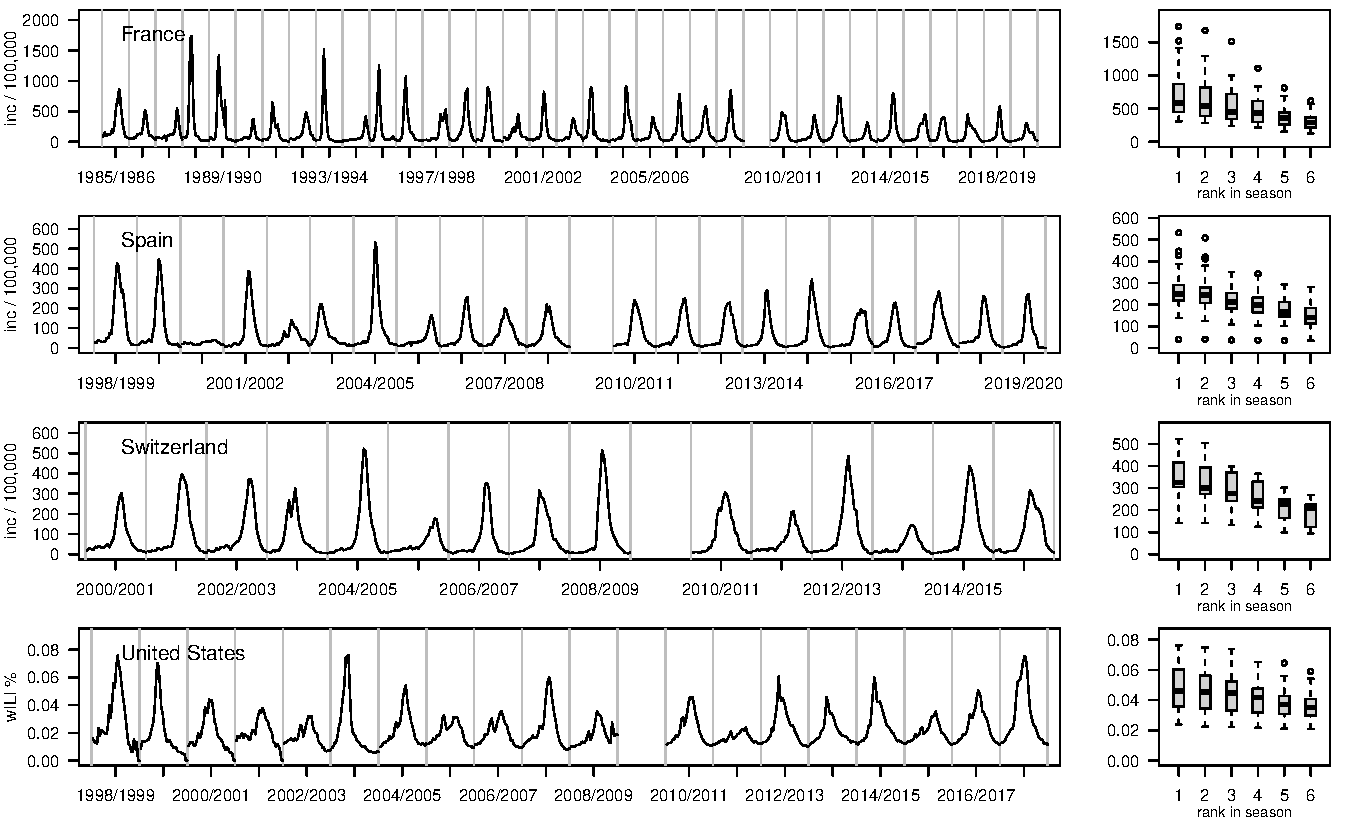
\includegraphics[width=0.9\textwidth]{figure/plot_data.pdf}

\subsection{Used software}

MEM version xxx, R software

\subsection{Results}

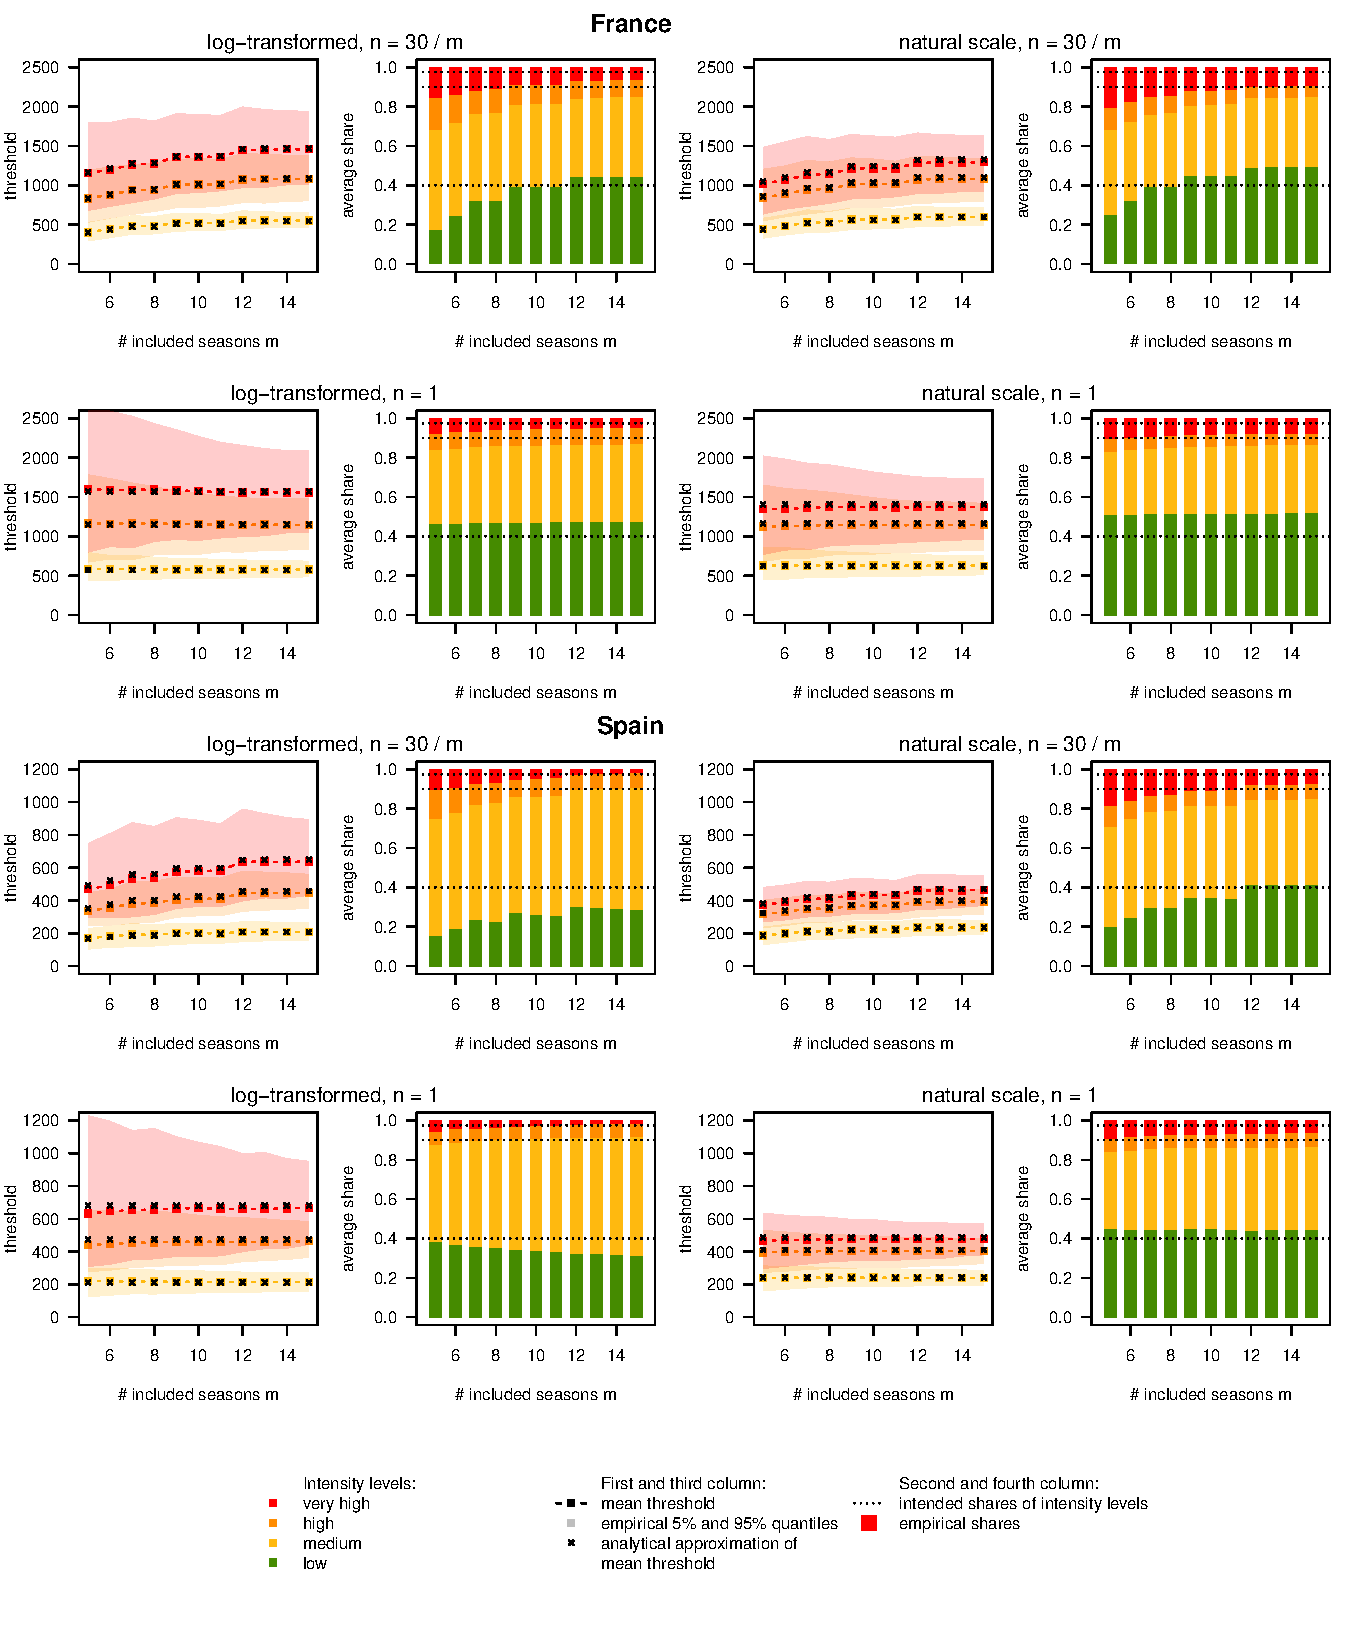
\includegraphics[page=1, width=0.9\textwidth]{figure/plot_results.pdf}

\includegraphics[page=2, width=0.9\textwidth]{figure/plot_results.pdf}


\section{Discussion}
\label{sec:discussion}

\section*{Outline of idea}

\begin{itemize}
\item Description of importance: officially embraced by ECDC
\item Describe other approaches, in particular WHO
\item Statistically correct description of what is being done, contract to WHO approach (which only uses peak -- good -- but uses normal rather than log-normal -- not so good. There is a PLOS paper where there is already a kind of combination of the two (WHO with log transformation))
\item Overview of how it is being used in the literature:
\begin{itemize}
\item How much training data was available in each study?
\end{itemize}
\item Simulation study based on permutation of true seasons:
\begin{itemize}
\item Countries: France, Switzerland, some third (European) country? Spain?
\item Important: standardize with time-varying population
\end{itemize}
\end{itemize}

\title{A statistical perspective on the moving epidemic method }
\author{Johannes Bracher}
\maketitle



\bibliographystyle{apalike}
\bibliography{bibliography_mem}
\end{document}